\subsubsection{FIDO2}

Fast Identity Online Alliance (\acrshort{fido} Alliance) is an organization developing authentication standards. Protocols like \acrfull{u2f}, \acrfull{uaf} or \acrshort{fido}2 are products of \acrshort{fido} Alliance and its partners. The main aim of \acrshort{fido} is to create phishing-proof, password-less and secure standards. \acrshort{u2f} and \acrshort{uaf} has been proposed in 2014(REF), both being updated and having new versions over time however, the focus will be put towards the newest \acrshort{fido}2 project and its specification rather than older standards.

The \acrshort{fido}2 project’s aim is to provide phishing-proof, password-less, secure and simple authentication protocol. Fundamental components of \acrshort{fido}2 are WebAuthn which is the \acrshort{api} for a client (by \acrshort{w3c}) and \acrshort{ctap} (by \acrshort{fido}), the \acrshort{api} for the authenticator. These define an abstraction layer which allows strongly authenticated credentials. Therefore, any supported client, being it a native application or browser, running on client’s device and any supported authenticator, being it a build in or roaming authenticator connected to the device via \acrshort{nfc}, \acrshort{ble} or \acrshort{usb}, can use a standardized method to authenticate the user. There are several entities involved in the process of registering and subsequently authenticating the user as it can be seen in Figure XY.

\begin{figure}[ht]
    \centering
    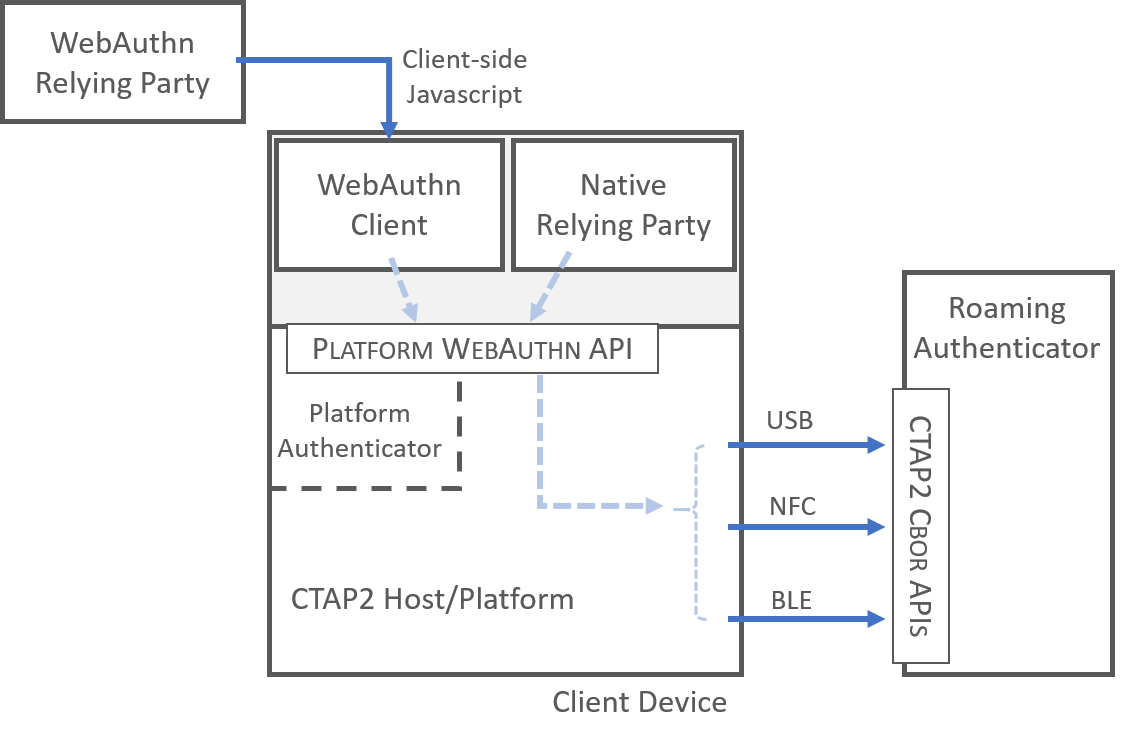
\includegraphics[width=.95\textwidth]{00images/FIDO2_Overview.png}
    \caption{Explanation. From~\cite{}SOURCE}
    \label{fig:fido2_overview}
\end{figure}

\subparagraph{Client Device:} 
is a hardware which is hosting the authentication via built in or roaming authenticator and communicates with a relying party. Example of such devices are laptops or smartphones. 

\subparagraph{Roaming Authenticator:} 
is an authenticator which can be connected to different client devices using \acrshort{ble}, \acrshort{nfc} or \acrshort{usb} interfaces. To communicate with a client device, \acrshort{ctap}1 or \acrshort{ctap}2 can be used.

\subparagraph{Platform Authenticator:} 
is built in on a client device and can only be used with a given device. Example of such authenticators are fingerprint scanners or facial recognition.

\subparagraph{Relaying Party:} 
is an application or service which requests authenticated credentials. It can be a native or web application.

\subparagraph{\acrshort{ctap}2:}
\acrlong{ctap} 2 (\acrshort{ctap}2) is the newest version of the \acrshort{ctap} protocol, which is backward compatible the preceding \acrshort{ctap}1/\acrshort{u2f} protocol by mapping \acrshort{ctap}2 request to \acrshort{ctap}1/\acrshort{u2f} and vice versa for responses, unless the relaying party requests a parameter which is \acrshort{ctap}2 specific. 

The \acrshort{ctap}2 specifies the application layer protocol so that authenticator and client device can communicate, as well as it defines how transport layer connection with different physical authenticators should be set up in accordance with the application layer protocol. This enables external devices to be used as authenticators and work with WebAuthn with applications and services.

The biggest improvements of \acrshort{ctap}2 over \acrshort{ctap} is the option to verify the user using biometrics or PIN. On top of that, besides storing a private key, devices are capable of storage of associated metadata which allows login even without typing an username. Android phones with android 7.0 and higher can be used as authenticators with their fingerprint or biometric scanners, thanks to a support of Trusted Platform Modules.(REF)

\subparagraph{WebAuth:} 
Web Atuthentication (WebAuthn) is the new web standard published on 4th March 2019  by \acrshort{w3c} which defines web \acrshort{api} which enables web browsers and platforms to enable external authenticators using \acrshort{fido} authentication. It standardizes the public-key authentication between users and web applications or services, so it is being used for communication between the client device and a RP.\\

When a user wants to use authentication with \acrshort{fido}2, given application or website must support it at first place. User can create a new account or use already existing one and associate it with the \acrshort{fido}2 authentication. The authenticator, whether it is a roaming or built-in one, creates cryptographic key pair (private and public key) on user request which has to be confirmed by a user gesture, e.g. fingerprint, biometrics, PIN, touch. Key pair is then created, and the private key is securely stored on the authenticator while the public one, along with associated account details is sent to a server for storage.

In figure XYZ below, the high level sequence diagram of \acrshort{fido}2 authentication is shown. When a user wants to log-in to a service the relying party sends Credential ID and a challenge to a client, which then forwards this data to authenticator along with Relying party ID and Token binding. In order to proceed with authentication, user's gesture is required. Relying party ID counters the man-in-the-middle attack making sure, that it is always the same party the authentication is done with. Having Credential ID allows to have multiple accounts associated with the same key for the same service and have different key pair for each of the accounts. Authenticator then look up the private key based on Credential ID and Relying party ID, which is then being used to sign the payload. The signed payload and the counter are sent then as an assertion to the client, which forwards it to the relying party together with the initial request. The relying party then verifies the signature with the public key of given account and logs in the user. Counter secures the authentication from clones of the authenticator. In case that the authenticators is cloned and now there are two of them, by having the counter, they only share the same history, but their futures divert, because at each payload signing the counter increments on the authenticator. Therefore, if the clones is used at some point, it has lower counter than the is supposed to and gets detected and user gets notified.

\begin{figure}[ht]
    \centering
    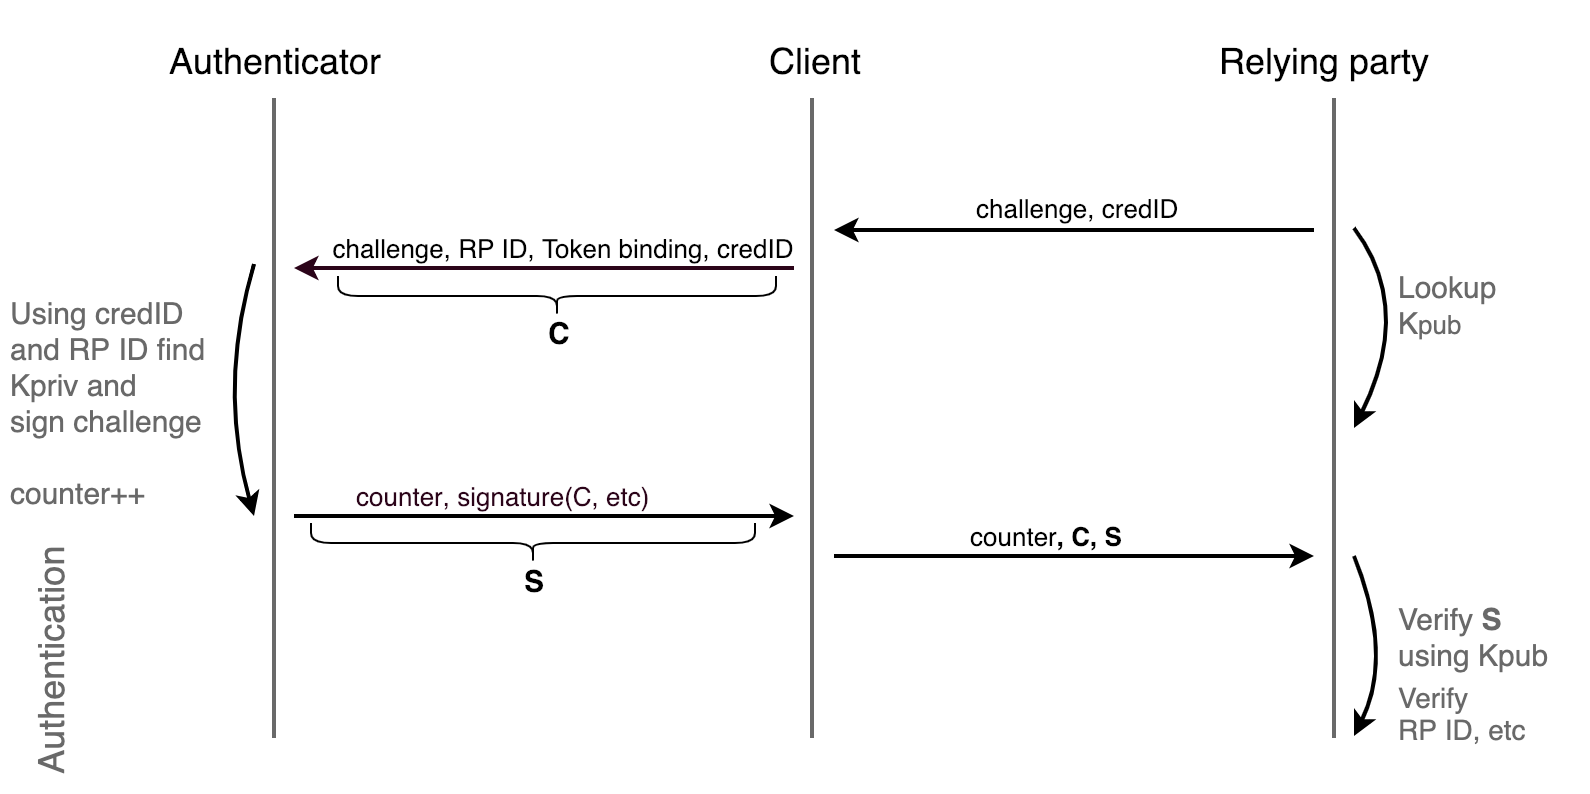
\includegraphics[width=.95\textwidth]{00images/FIDO2_Authentication.png}
    \caption{Explanation. From~\cite{}SOURCE}
    \label{fig:fido2_authentication}
\end{figure}